\documentclass[11pt,a4paper]{article}
\usepackage[margin=1in]{geometry}
\usepackage{hyperref}
\usepackage{enumitem}
\usepackage{graphicx}
\usepackage{xcolor}
\usepackage{amsmath}
\usepackage{amssymb}
\usepackage{booktabs}
\usepackage{tikz}
\usetikzlibrary{shapes.geometric, arrows, positioning}

\title{\textbf{SOFTWARE REQUIREMENTS SPECIFICATION}\\[0.5em]
\Large for\\[0.5em]
\Huge \textbf{ESTATEPULSE}\\[0.3em]
\Large Real Estate Price Prediction and Marketplace Platform\\[0.2em]
\small (Academically Cataloged as PropertyPulse in UCS503 Records)\\[1em]
\normalsize Version 1.0}

\author{
  \textbf{Prepared by:}\\[0.5em]
  1. Guntaas Singh \quad (\texttt{1024030108})\\
  2. Haneesh \quad (\texttt{1024030112})\\
  3. Dhruv Rajput \quad (\texttt{1024030538})\\
  4. Atiksh Gupta \quad (\texttt{102303133})\\[0.8em]
  \textit{Group: 3C14, BE Third Year, Computer Engineering (COE)}\\[1.5em]
  \textbf{Submitted to:}\\
  Ms. Anushka\\
  \textit{Lecturer / Course Instructor}\\
  \textit{Computer Science and Engineering Department}\\
  \textit{Thapar Institute of Engineering and Technology, Patiala}
}

\date{October 2026}

\begin{document}

\maketitle
\thispagestyle{empty}
\newpage

\tableofcontents
\newpage

\section{Introduction}

\subsection{Purpose}
In traditional real estate transactions, prospective buyers and sellers suffer from acute information asymmetry, fragmented communication across unlinked third-party channels, opaque pricing, and duplicate property advertisements. 

The purpose of this \textbf{Software Requirements Specification (SRS)} is to provide a formal, rigorous, and verifiable specification for \textbf{EstatePulse} (cataloged as \textit{PropertyPulse} in institutional records). EstatePulse is an AI-driven real estate marketplace and predictive valuation web application engineered for the \textbf{UCS 503 (Software Engineering)} course at Thapar Institute of Engineering and Technology. This document establishes all functional modules, non-functional quality attributes, mathematical models, system architecture, and operational constraints governing the implementation.

\subsection{Intended Audience and Reading Suggestions}
This document is structured for the following stakeholders:
\begin{itemize}[leftmargin=0.8cm]
    \item \textbf{Course Instructor and Academic Evaluators (Ms. Anushka):} To evaluate alignment with approved proposal objectives, architectural soundness, and software engineering rigor.
    \item \textbf{Development Team:} To guide implementation across the 3-tier architecture, API endpoint contracts, ML pipeline, and responsive front-end.
    \item \textbf{Software Verification and Test Engineers:} To construct unit, integration, and user-acceptance test suites.
\end{itemize}

\subsection{Project Scope}
EstatePulse unifies property discovery, pricing intelligence, and buyer-seller negotiations:
\begin{enumerate}[leftmargin=0.8cm]
    \item \textbf{Property Listing Portal with Instant ML Valuation:} Sellers submit listings specifying structural dimensions, locality, and furnishings. The system generates an immediate market valuation ($\hat{y}$) and performs automated duplicate checks.
    \item \textbf{Buyer Barometer:} An algorithmic visual indicator categorizes listings into \textit{Great Deal}, \textit{Fair Market Price}, or \textit{Premium} based on statistical price variance.
    \item \textbf{Integrated Negotiation Chat:} A WhatsApp-like in-app messaging channel per property, eliminating fragmented third-party communication.
    \item \textbf{Site Visit Scheduling \& Escrow Token:} Formal appointment booking for site inspections accompanied by booking token checkout.
    \item \textbf{Empirical Metric Attribution:} Instruments and reports the \textbf{Time-to-Appointment} metric ($T_{\text{appt}} = t_{\text{confirmed}} - t_{\text{inquiry}}$) with a benchmark target of $\le 2$ hours.
\end{enumerate}

\begin{figure}[htbp]
\centering
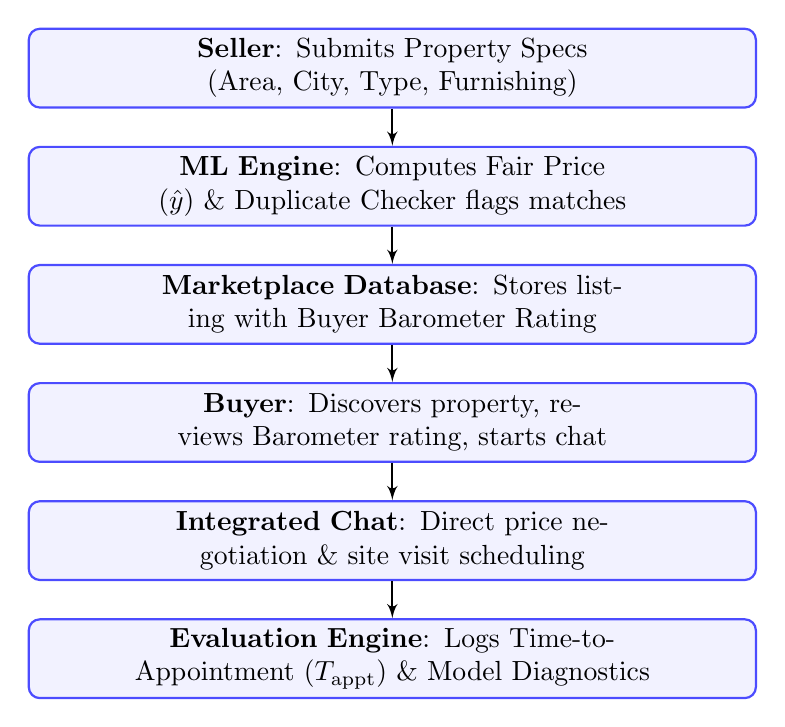
\begin{tikzpicture}[node distance=1.5cm, auto,
    block/.style={rectangle, draw=blue!70, fill=blue!5, thick, text width=9cm, text centered, rounded corners, minimum height=1cm},
    line/.style={draw, -latex', thick}]
    \node [block] (seller) {\textbf{Seller}: Submits Property Specs (Area, City, Type, Furnishing)};
    \node [block, below of=seller] (ml) {\textbf{ML Engine}: Computes Fair Price ($\hat{y}$) \& Duplicate Checker flags matches};
    \node [block, below of=ml] (catalog) {\textbf{Marketplace Database}: Stores listing with Buyer Barometer Rating};
    \node [block, below of=catalog] (buyer) {\textbf{Buyer}: Discovers property, reviews Barometer rating, starts chat};
    \node [block, below of=buyer] (chat) {\textbf{Integrated Chat}: Direct price negotiation \& site visit scheduling};
    \node [block, below of=chat] (eval) {\textbf{Evaluation Engine}: Logs Time-to-Appointment ($T_{\text{appt}}$) \& Model Diagnostics};

    \path [line] (seller) -- (ml);
    \path [line] (ml) -- (catalog);
    \path [line] (catalog) -- (buyer);
    \path [line] (buyer) -- (chat);
    \path [line] (chat) -- (eval);
\end{tikzpicture}
\caption{Entire System Workflow}
\label{fig:workflow}
\end{figure}

\newpage
\section{Overall Description}

\subsection{Product Perspective}
EstatePulse operates as an autonomous, self-contained 3-tier web platform:
\begin{itemize}[leftmargin=0.8cm]
    \item \textbf{Client / Presentation Tier:} Single Page Application (SPA) developed in semantic HTML5, modern CSS3, and Vanilla JavaScript (ES6+), optimized for both mobile and desktop viewports.
    \item \textbf{Application \& ML Tier:} Lightweight Python Flask REST API integrating Scikit-learn multiple linear regression and duplicate text detection.
    \item \textbf{Persistence Tier:} SQLite relational database storing normalized tables for users, listings, messages, appointments, and payments.
\end{itemize}

\subsection{User Classes and Characteristics}
\begin{itemize}[leftmargin=0.8cm]
    \item \textbf{Guest User:} Unauthenticated visitor with read-only access to browse and filter marketplace listings and inspect Buyer Barometer ratings.
    \item \textbf{Buyer:} Authenticated user capable of initiating chat threads, bookmarking properties, scheduling site visits, and submitting booking tokens.
    \item \textbf{Seller:} Authenticated property owner or broker empowered to list real estate, receive instant ML valuations, review duplicate alerts, chat with buyers, and confirm visit appointments.
    \item \textbf{Evaluator / Administrator:} Academic instructor or administrator accessing diagnostic telemetry, ML residual metrics ($R^2$, MSE, RMSE), and time-to-appointment histograms.
\end{itemize}

\subsection{Product Functions}
The principal functional capabilities encompass:
\begin{enumerate}[leftmargin=0.8cm]
    \item \textbf{Machine Learning Property Valuation:} Multivariate regression over physical property dimensions and regional weights.
    \item \textbf{Duplicate Listing Detection:} Similarity analysis on category, locality, and dimensional bounds to prevent spam.
    \item \textbf{Buyer Barometer Categorization:} Automated calculation of price deviation percentages.
    \item \textbf{Contextual Negotiation Chat:} Property-isolated messaging channels.
    \item \textbf{Site Visit Scheduling \& Escrow Token:} Structured appointment state machine and payment token recording.
    \item \textbf{System Evaluation Instrumentation:} Automated timestamp calculation for empirical metrics.
\end{enumerate}

\subsection{Operating Environment}
\begin{itemize}[leftmargin=0.8cm]
    \item \textbf{Host Environment:} Windows 10/11, Ubuntu Linux 20.04+, macOS.
    \item \textbf{Software Requirements:} Python 3.10+, Flask 3.x, Scikit-learn 1.4+, SQLite 3.
    \item \textbf{Client Web Browsers:} Google Chrome 110+, Mozilla Firefox 115+, Apple Safari 16+, Edge, Mobile Safari/Chrome.
    \item \textbf{Hardware Constraints:} Memory footprint $< 120$ MB during active inference; server executable on modest 1 vCPU / 512 MB virtual environments.
\end{itemize}

\subsection{Design Activities}
The operational lifecycle partitions into:
\begin{itemize}[leftmargin=0.8cm]
    \item \textbf{Buyer Flow:} Browse $\rightarrow$ Filter $\rightarrow$ Evaluate Barometer $\rightarrow$ Chat Inquiry $\rightarrow$ Book Inspection $\rightarrow$ Pay Token.
    \item \textbf{Seller Flow:} Enter Specifications $\rightarrow$ Live ML Valuation $\rightarrow$ Duplicate Validation $\rightarrow$ Publish Listing $\rightarrow$ In-App Negotiation $\rightarrow$ Confirm Visit.
    \item \textbf{Diagnostics Flow:} Timestamp Capture ($t_{\text{inquiry}}, t_{\text{confirmed}}$) $\rightarrow$ Duration Delta Calculation $\rightarrow$ Median Aggregation $\rightarrow$ Live Console Display.
\end{itemize}

\newpage
\section{System Features}

\subsection{Description and Priority}
\begin{table}[htbp]
\centering
\begin{tabular}{@{}llll@{}}
\toprule
\textbf{Priority} & \textbf{ID} & \textbf{Feature Name} & \textbf{Operational Status} \\ \midrule
High (P1) & FEAT-01 & ML Price Predictor Engine & Implemented \\
High (P1) & FEAT-02 & Property Listing \& Duplicate Detection & Implemented \\
High (P1) & FEAT-03 & Buyer Barometer Visual Guidance & Implemented \\
High (P1) & FEAT-04 & In-App WhatsApp-Style Negotiation Chat & Implemented \\
Medium (P2) & FEAT-05 & Appointment Scheduling \& Token Payment & Implemented \\
Medium (P2) & FEAT-06 & Role-Based Auth \& Guest Browsing & Implemented \\
Low (P3) & FEAT-07 & System Diagnostics \& Attribution Dashboard & Implemented \\ \bottomrule
\end{tabular}
\caption{System Feature Prioritization Matrix}
\label{tab:features}
\end{table}

\subsection{Functional Requirements (Module Breakdown)}

\subsubsection{Module 1: Property Listing and Duplicate Detection (FEAT-02)}
\begin{itemize}[leftmargin=0.8cm]
    \item \textbf{FR-1.1:} The system shall accept property listings with attributes: Title, Description, Property Type (\textit{Residential, Commercial, Apartment, Villa, Entertainment}), City, Locality, Area (sq.ft), Bedrooms, Bathrooms, Age (years), Parking, Furnishing, and Asking Price (INR).
    \item \textbf{FR-1.2:} Mandatory client-side and server-side validation shall ensure positive values for area and price.
    \item \textbf{FR-1.3:} On submission, the backend shall query the active database to detect duplicate submissions matching the same locality, category, and area range ($\pm 5\%$).
\end{itemize}

\subsubsection{Module 2: Machine Learning Price Prediction (FEAT-01)}
\begin{itemize}[leftmargin=0.8cm]
    \item \textbf{FR-2.1:} As property specifications are modified, the front-end shall invoke \texttt{POST /api/predict} (debounced at 300ms) to compute $\hat{y}$.
    \item \textbf{FR-2.2:} The prediction engine shall convert qualitative attributes into one-hot encoded feature vectors and return: \texttt{predicted\_price}, \texttt{barometer\_score}, \texttt{barometer\_verdict}, and \texttt{advice}.
\end{itemize}

\subsubsection{Module 3: Buyer Barometer Visualizer (FEAT-03)}
\begin{itemize}[leftmargin=0.8cm]
    \item \textbf{FR-3.1:} The system shall calculate price deviation:
    $$\Delta\% = \left(\frac{P_{\text{asking}} - P_{\text{predicted}}}{P_{\text{predicted}}}\right) \times 100$$
    \item \textbf{FR-3.2:} Listings with $\Delta\% \le -10\%$ shall display a \textbf{Great Deal} green badge; $-10\% < \Delta\% \le +10\%$ shall display a \textbf{Fair Market Price} blue badge; $\Delta\% > +10\%$ shall display a \textbf{Premium / High} warning badge.
\end{itemize}

\subsubsection{Module 4: Integrated Negotiation Chat (FEAT-04)}
\begin{itemize}[leftmargin=0.8cm]
    \item \textbf{FR-4.1:} Each property shall possess an isolated messaging thread mapped by \texttt{property\_id}.
    \item \textbf{FR-4.2:} Messaging endpoints (\texttt{POST /api/properties/<id>/messages} and \texttt{GET}) shall support thread synchronization via 3-second client polling.
    \item \textbf{FR-4.3:} The arrival of the initial buyer inquiry shall log the \texttt{first\_inquiry\_timestamp}.
\end{itemize}

\subsubsection{Module 5: Site Visit Scheduling and Token Payment (FEAT-05)}
\begin{itemize}[leftmargin=0.8cm]
    \item \textbf{FR-5.1:} Buyers shall reserve inspection dates ($\ge \text{tomorrow}$) and specify slot times.
    \item \textbf{FR-5.2:} The appointment flow shall invoke \texttt{POST /api/payments} to record visit token transactions.
    \item \textbf{FR-5.3:} Seller confirmation shall update appointment status to \texttt{confirmed} and compute duration:
    $$\text{time\_to\_appointment\_seconds} = t_{\text{confirmed}} - t_{\text{first\_inquiry}}$$
\end{itemize}

\subsubsection{Module 6: System Diagnostics and Metrics (FEAT-07)}
\begin{itemize}[leftmargin=0.8cm]
    \item \textbf{FR-6.1:} Expose \texttt{GET /api/metrics} reporting median Time-to-Appointment across all closed appointments.
    \item \textbf{FR-6.2:} Display model validation metrics: $R^2$ score, Mean Squared Error (MSE), and Root Mean Squared Error (RMSE).
\end{itemize}

\newpage
\section{Other Nonfunctional Requirements}

\subsection{Performance Requirements}
\begin{itemize}[leftmargin=0.8cm]
    \item \textbf{ML Prediction Latency:} Predictive model inference response time $< 100$ ms.
    \item \textbf{Page Response Time:} Initial DOM interactive load time $< 1.5$ seconds.
    \item \textbf{Query Latency:} Database listing queries execute in $< 50$ ms.
    \item \textbf{SLA Target:} Median Time-to-Appointment maintained $\le 2$ hours during pilot operations.
\end{itemize}

\subsection{Security Requirements}
\begin{itemize}[leftmargin=0.8cm]
    \item \textbf{SQL Injection Prevention:} Mandatory use of parameterized queries across all SQLite interactions.
    \item \textbf{XSS Mitigation:} Strict sanitization and HTML escaping of user inputs prior to rendering.
    \item \textbf{Access Control:} Role enforcement ensuring sellers may only manage their respective listings.
\end{itemize}

\subsection{Software Quality Attributes}
\begin{itemize}[leftmargin=0.8cm]
    \item \textbf{Usability \& High Contrast:} Mobile-responsive layout conforming to touch target criteria ($\ge 44 \times 44$ px) with high-contrast text typography.
    \item \textbf{Reliability:} $\ge 99\%$ uptime during designated course evaluation windows.
    \item \textbf{Maintainability:} Strict architectural separation between database logic (\texttt{database.py}), ML pipeline (\texttt{ml_model.py}), and web routing (\texttt{app.py}).
\end{itemize}

\subsection{Business Rules \& Mathematical Specifications}
Price estimation is governed by the Multiple Linear Regression equation:
$$\hat{y} = \beta_0 + \sum_{i=1}^{n} \beta_i x_i + \epsilon$$
Evaluated with Mean Squared Error (MSE):
$$\text{MSE} = \frac{1}{n} \sum_{i=1}^{n} (y_i - \hat{y}_i)^2$$

\section{Other Requirements and Constraints}
\begin{itemize}[leftmargin=0.8cm]
    \item \textbf{Educational Constraint:} Execution within self-contained Python virtual environment without reliance on external commercial paid APIs.
    \item \textbf{Deployability:} Standardized configuration suitable for immediate deployment across local academic laboratories or free-tier hosting platforms.
    \item \textbf{Future Extensions:} Bi-directional WebSocket communication (Socket.IO) and image deduplication via convolutional perceptual hashing.
\end{itemize}

\end{document}
